\documentclass[handout]{beamer}

\usepackage{fontspec} 
% \usepackage{lsp-makros}
\useoutertheme{lsp}

\usepackage{lsptitle}

\def\two@digits#1{\ifnum#1<10 0\fi\number#1}
\def\mytoday{\two@digits{\number\day}.\two@digits{\number\month}.\number\year}


\usepackage{xspace,multicol}
\newcommand{\latex}{\LaTeX\xspace}
\usepackage{tikz}


\newcounter{lastpagemainpart}
\footnotesep0pt
\renewcommand{\footnoterule}{}
\usefootnotetemplate{
  \noindent
  \insertfootnotemark\insertfootnotetext}

\let\beamerfn=\footnote
\renewcommand{\footnote}[1]{%
\let\oldfnsize=\footnotesize%
\let\footnotesize=\tiny%
\beamerfn<\thebeamerpauses->{#1}%
\let\footnotesize=\oldfnsize}


\date{\today}

\usepackage{eurosym}  
 
\renewcommand{\centerline}[1]{\hfill#1\hfill\hfill\mbox{}}


\title{Reviewing}
% \institute{FU Berlin}
\author[LangSci]{Language Science Press}



\begin{document}
\lspbeamertitle

\section{Timeline}
\frame{
\frametitle{Timeline}
%   \includegraphics[height=.2\textheight]{./path/to/graphicsfile}
  \begin{enumerate}
    \item   expression of interest (informal)
    \begin{itemize}
      \item please forward them to the LangSci office for bookkeeping
    \end{itemize}
    \item[{1.\parbox{0mm}{\small{$^{'}$}}}]   proposal (formal)
    \item   manuscript submission
    \item   revised version
    \item   published version
  \end{enumerate}
}

\section{Outcomes}
\frame{
\frametitle{Outcomes}
%   \includegraphics[height=.2\textheight]{./path/to/graphicsfile}
  \begin{itemize}
    \item  desk rejection of EoI/proposal
    \item  rejection of submitted manuscript
    \begin{itemize}
      \item possibility to resubmit after 1 year
    \end{itemize}
    \item  acceptance with revisions
    \begin{itemize}
     \item  \textbf{you} are the editor, you decide
     \item it is OK to overrule reviewers
    \end{itemize}
  \end{itemize}
}


\section{Document types}
\frame{
\frametitle{Reviewing monographs}
  \begin{itemize}
    \item  monographs
    \begin{itemize}
      \item classical review
      \item open review
    \end{itemize}
    \end{itemize}
    }


\frame{
\frametitle{Reviewing grammars}
    \begin{itemize}
      \item classical review
      \item optional ``distributed review''
      \begin{itemize}
        \item chapter on phonology goes to a phonologist
        \item chapter on syntax goes to a syntactician
        \item ...
      \end{itemize}
    \end{itemize}
    }

\frame{
\frametitle{Edited volumes}
    \begin{itemize}
      \item proposal review
        \begin{itemize}
          \item check focus
          \item drop some chapters
          \item invite further chapters
        \end{itemize}
      \item submission review
      \begin{itemize}
      \item complex vetting context with volume editors and series editors
      \begin{enumerate}
        \item \textbf{delegated review}: series editors trust volume editors
        \item \textbf{compliance review}: series editors check that volume editors respected procedures but do not check content
        \item \textbf{early two-reviews system}: all chapter reviews go to series editors, who then decide about acceptance
        \item \textbf{late two-reviews system}: all revised chapters go to series editors, who then decide about acceptance
      \end{enumerate}
      \item often 1 internal and 1 external review per chapter
      \item see {\small\url{https://userblogs.fu-berlin.de/langsci-press/2016/02/08/reviewing-of-edited-volumes}}
      \end{itemize}
  \end{itemize}
}


\section{Review formats}
\frame{
\frametitle{Formats}
%   \includegraphics[height=.2\textheight]{./path/to/graphicsfile}
  \begin{itemize}
    \item  Closed review (traditional)
    \item  Disclosed review (reviews and reviewer identities are disclosed after acceptance)
    \item Open review (anybody can comment)
  \end{itemize}
}

\frame{
\frametitle{\mbox{Disclosed review and open review}}
\begin{tabular}{c||c}
    Disclosed review & Open review on PaperHive \\
    \hline
  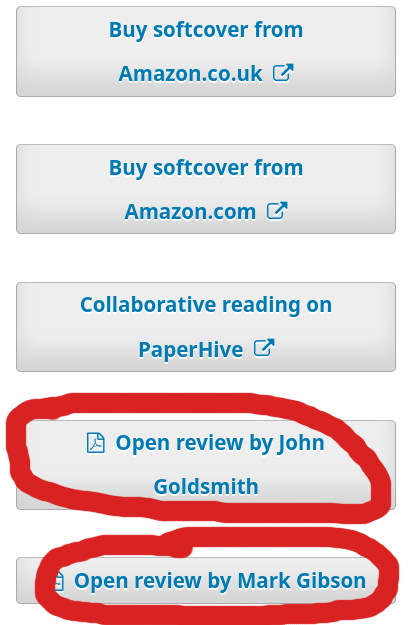
\includegraphics[height=.8\textheight]{tilsen.png} &
  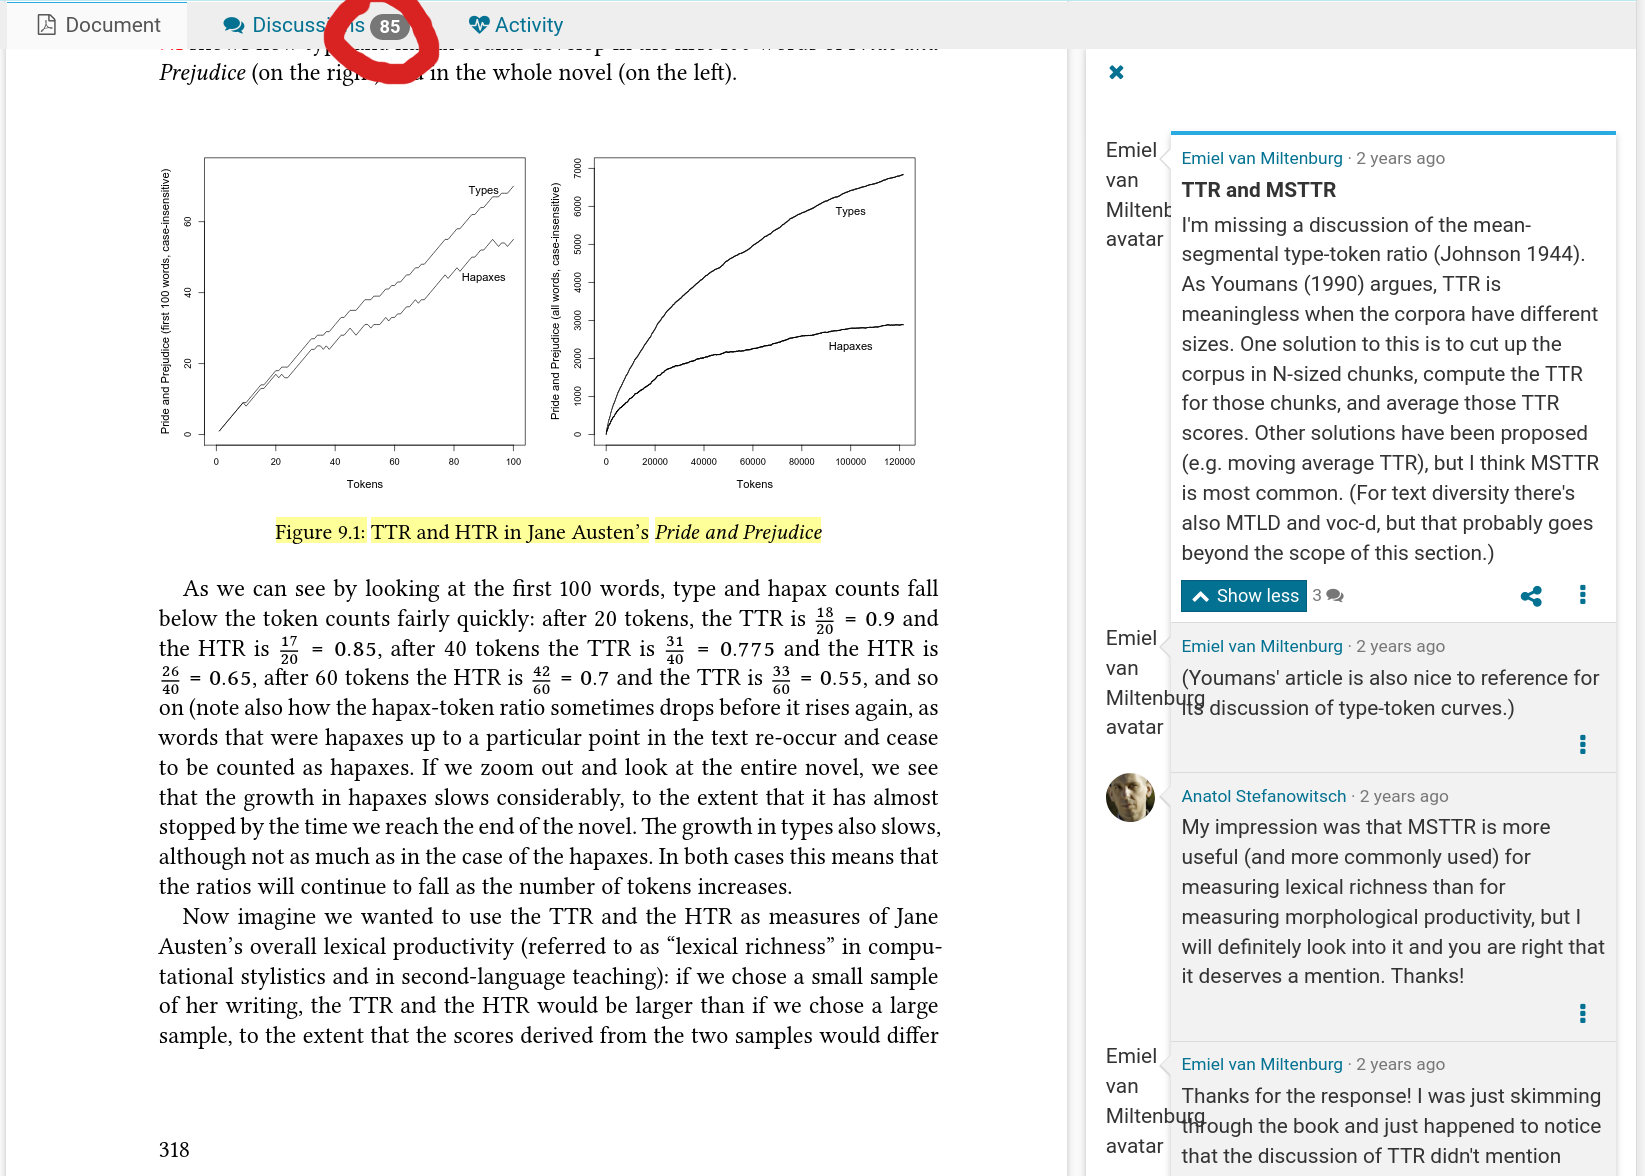
\includegraphics[height=.8\textheight]{stefanowitsch.png}
  \end{tabular}

}

\frame{
\frametitle{Discussion}
  \begin{itemize}
    \item  recruiting reviewers?
    \item  edited volumes?
    \item open reviewing?
  \end{itemize}
}

%\setcounter{framenumber}{\thelastpagemainpart}
\end{document}
